
Attention now turns to the assessment of ASV vulnerabilities to replay spoofing, which are shown to be comparable to those of voice conversion and speech synthesis.  These findings motivate the assessment of replay countermeasures.


\subsection{Replay spoofing}


\begin{figure}[!t]
	\centering
	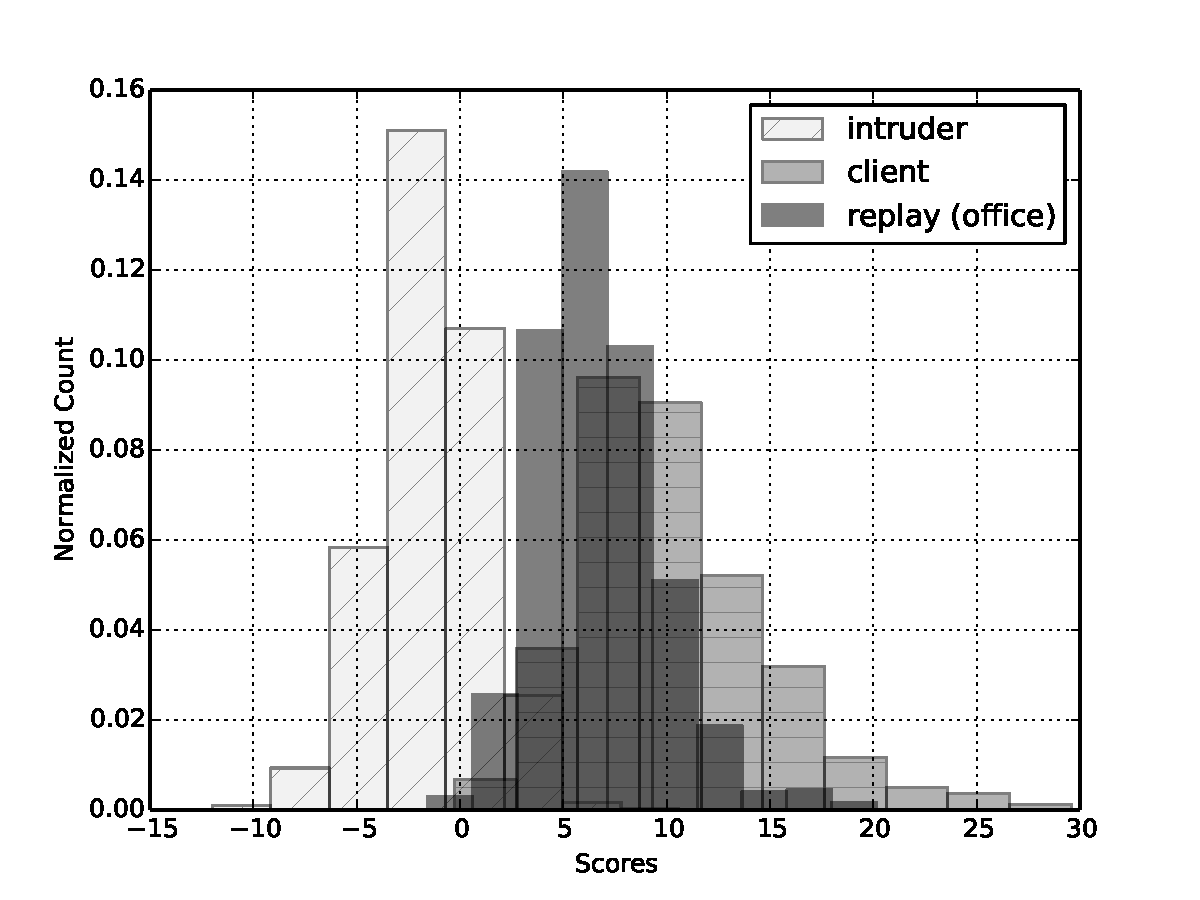
\includegraphics[width=1\linewidth]{Figs/dist_IV_off.pdf}
	\caption{Score distribution for the IV-PLDA system for replay attacks using a stand-alone speaker and emulation of an office.}
	\label{fig::Dist_IV}
\end{figure}


% distributions
Fig.~\ref{fig::Dist_IV} shows the effect of replay attacks on the score distributions for the IV-PLDA system.  While the zero-effort impostor and genuine client distributions are well separated, the latter overlaps significantly with the score distribution for replay attacks collected in an office environment.  Increased overlap between these distribution will degrade ASV performance.


\begin{figure}[!t]
	\centering
	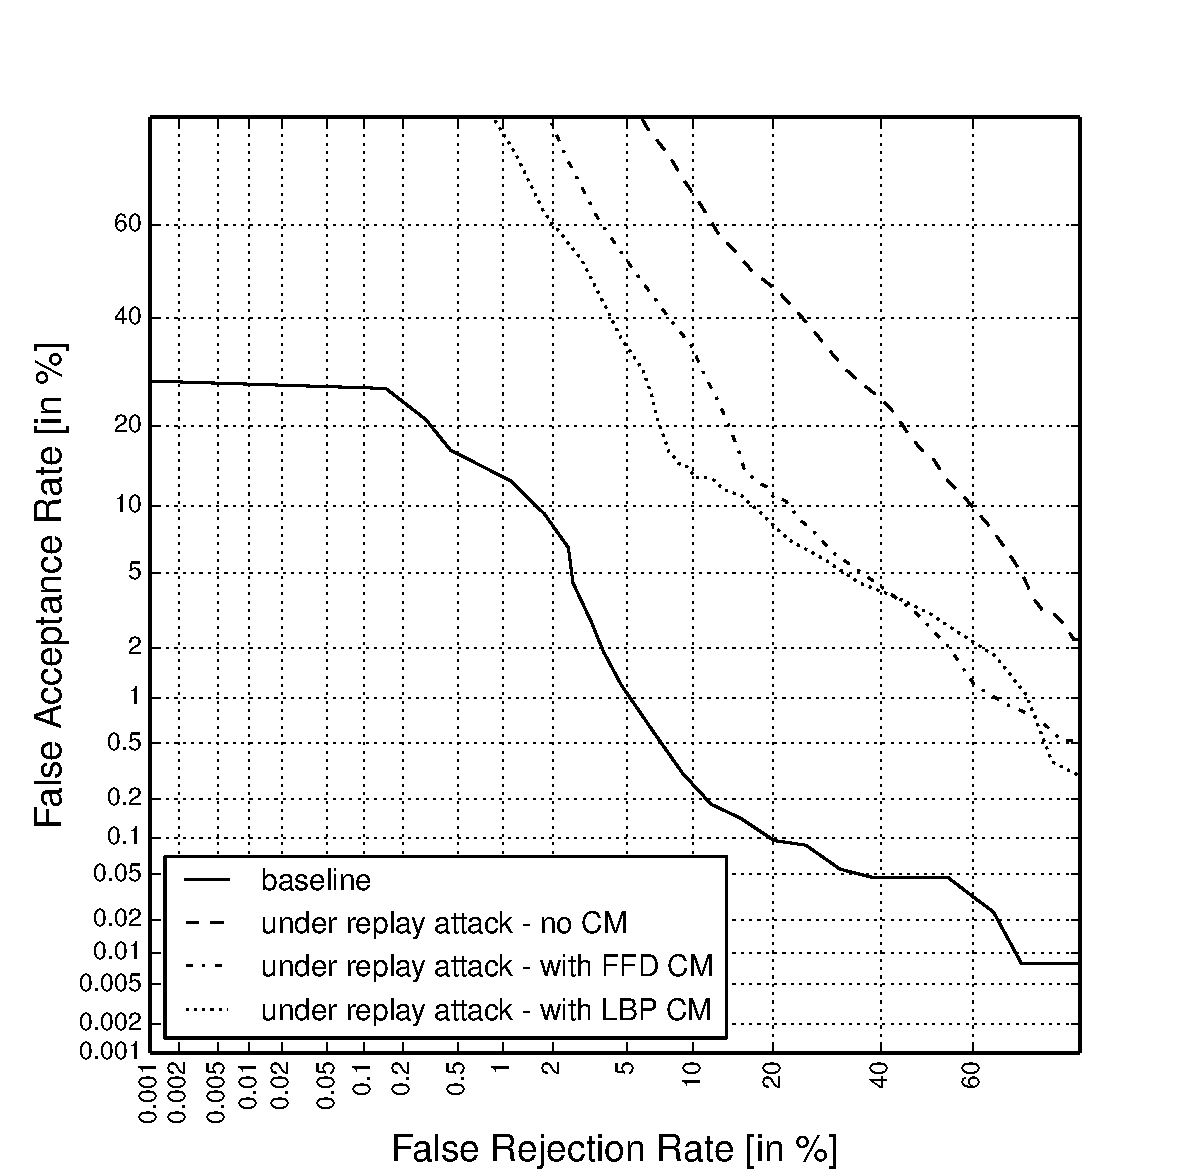
\includegraphics[width=1\linewidth]{Figs/DET_IVPLDA_counter_Behr.pdf}
	\caption{DET plots for the IV-PLDA system: (i) the baseline, (ii) under replay spoofing with a stand-alone speaker in an office, (iii) under replay attack, but with FFD and (iv) LBP countermeasures - to be referred to later.}

%% {\bfseries There is too much information on this plot.  I suggest to include only four profiles: (i) the baseline, (ii) spoofing under the same conditions as in Fig.~\ref{fig::Dist_IV} and (iii) and (iv) with FFD and LBP countermeasures - to be referred to later.}}
	\label{fig::DETs_replay_IV}
\end{figure}


% DET plots
Fig.~\ref{fig::DETs_replay_IV} illustrates a detection error trade-off (DET) plot\footnote{The DETs in this paper were produced with the TABULA RASA Scoretoolkit (http://publications.idiap.ch/downolads/reports/2012/Anjos\_Idiap-Com-02-2012.pdf) and the Bosaris toolkit (https://sites.google.com/site/bosaristoolkit/).} for the same experimental setup.  The lower-most, solid profile illustrates the performance of the baseline ASV system.  The upper-most profile illustrates performance when zero-effort impostors are replaced with replay attacks.  Thus, the difference between these two profiles serves as an indication of the system vulnerability to replay spoofing; in this case the degradation in performance is significant.  


\begin{table*}
\renewcommand{\arraystretch}{1.2}
\begin{center}
%    \begin{tabular}{ l l || c c c c c c c}
    \begin{tabular}{ l  c c c c c c c}
    \hline
%Score norm & Replay env. &  GMM & SGL & SGL-NAP  & SGL-FA & FA & IV & IV-PLDA \\ 
 &  GMM & SGL & SGL-NAP  & SGL-FA & FA & IV & IV-PLDA \\ 
 \hline \hline
%& (Baseline) & 9.08 & 7.89 & 6.35 & 6.08 & 5.60 & 6.67 & 3.20\\
%No & Office  & 40.26 & 34.43 & 33.52 & 30.72 & 33.85 & 27.83 & 29.11\\
%norm & Corridor & 35.71 & 28.24 & 28.53 & 25.75 & 29.92 & 23.02 & 22.78\\
%& None & 51.59 & 49.64 & 49.49 & 49.73 & 49.37 & 49.38 & 49.37\\
%\hline
%& (Baseline) & 8.63 & 8.13 & 6.31 & 5.72 & 5.61 & 6.72 & 2.98\\
%With & Office  & 60.32 & 92.98 & 29.92 & 28.54 & 30.12 & 28.89 & 30.30\\
%norm & Corridor & 55.91 & 88.20 & 23.59 & 21.62 & 24.97 & 23.31 & 24.53\\
%& None & 64.40 & 96.67 & 49.44 & 49.31 & 49.67 & 49.06 & 49.46\\
Baseline & 8.63 & 8.13 & 6.31 & 5.72 & 5.61 & 6.72 & 2.98\\
\hline
Replay: office environment & 60.32 & 92.98 & 29.92 & 28.54 & 30.12 & 28.89 & 30.30\\
Replay: corridor environment & 55.91 & 88.20 & 23.59 & 21.62 & 24.97 & 23.31 & 24.53\\
Replay: anechoic environment & 64.40 & 96.67 & 49.44 & 49.31 & 49.67 & 49.06 & 49.46\\
\hline
Voice conversion & 33.69 & 36.92 & 27.58 & 23.97 & 23.96 & tbc. & 19.30\\
Speech synthesis & 27.29 & 15.04 & 13.78 & 11.91 & 16.22 & tbc. & 10.82\\
\hline
    \end{tabular}
%    \caption{EER values for different ASV systems for various acoustic %environment of replay attacks, with and without score normalisation. }
    \caption{Equal error rates (EERs) for seven different ASV systems and for zero-effort impostors (baseline) and three different replay attack configurations (three different acoustic environments).  Results are averaged across the three different loudspeaker configurations.}
		\label{tab::results_EER}
   \end{center}

\end{table*}


% EER table described
This trend is repeated across the full set of seven ASV systems and different replay attack configurations;  
results are illustrated in Table~\ref{tab::results_EER}.
Results in the second row show the baseline performance for each ASV system and for only zero-effort impostors.
As expected, the IV-PLDA system delivers the lowest EER.

Rows 2--5 illustrate the degradation in performance when zero-effort impostors are replaced with replay attacks.
EERs are here averaged across the three loudspeaker configurations; other results not reported here showed greater sensitivity to the acoustic environment than to the loudspeaker characteristics.  
The performance of all seven systems degrades significantly.
The EER of the most sensitive GSL system increases from 8\% to in the order of 90\% for all three acoustic environments.
Even the EER of the most resistant SGL-FA system increases to between 22\% and 50\%.  
Finally, the EER of the state-of-the-art IV-PLDA system increases to between 25\% and 50\%.  

%, the EER increases systemthe  is  are shown to be severely sensitive to replay attacks. Even for the highly-reverberant corridor and the most resistant (in terms of EER) GSL kernel system with factor analysis and with T-norm, the EER rose to more than 22\% compared to the baseline 5.7\%. What was already visible in the DET plots (see Fig.~\ref{fig::DETs_replay_IV}), the results for the office are much worse -- the most resistant IV system (without PLDA and without score normalisation) and GSL-FA systems yielded the EER of ca. 28\%, whilst the other systems returned EERs of 30\% and more. If acoustic conditions are not emulated, the spoofing is almost perfect and the ASV systems yield EER values of 50\% or even more. 


%They show that all replay attacks caused a significant degradation of the ASV performance. However, there are major differences in ASV performance depending on acoustic environment. If the acoustic environment is omitted, the ASV system is almost ideally spoofed -- the DET lines are close to straight, with the EER values close to 50\%. In realistic cases, when the room acoustics is taken into account, the spoofing is slightly less severe. It can be easily observed that the ASV performance under replay attack in a corridor is better than in an office, probably due to higher level of reverberation for the corridor.


%\subsection{Replay speaker}

%In contrast, despite major differences in speakers' impulse responses (see Fig.~\ref{fig::IRs}), the differences between the DET plots corresponding to different speakers are only minor. It suggests a relatively low impact of a replay device on the effectiveness of replay attack. Since all seven ASV systems tested showed similar behaviour, therefore, for the sake of clearness, the next results will present the average of the three speakers used in experiments.




%\subsection{Effect of channel compensation}

%It is noteworthy that under replay attack the iVector system with probabilistic linear discriminant analysis (PLDA) often shows worse results than the iVector system alone, even though the PLDA significantly decreases the EER for the baseline system (from 6.7\% down to less than 3\%, with score normalisation). This can be explained that in normal conditions the PLDA improves the performance of iVector-based ASV system as it compensates the intersession differences caused by channel or speaker variation. However, in the case of replay attack this can be disadvantageous, because it also seems to compensate the differences caused by replay devices and replay environments.

%\begin{figure}
%	\centering
%	\begin{minipage}{.5\textwidth}
%	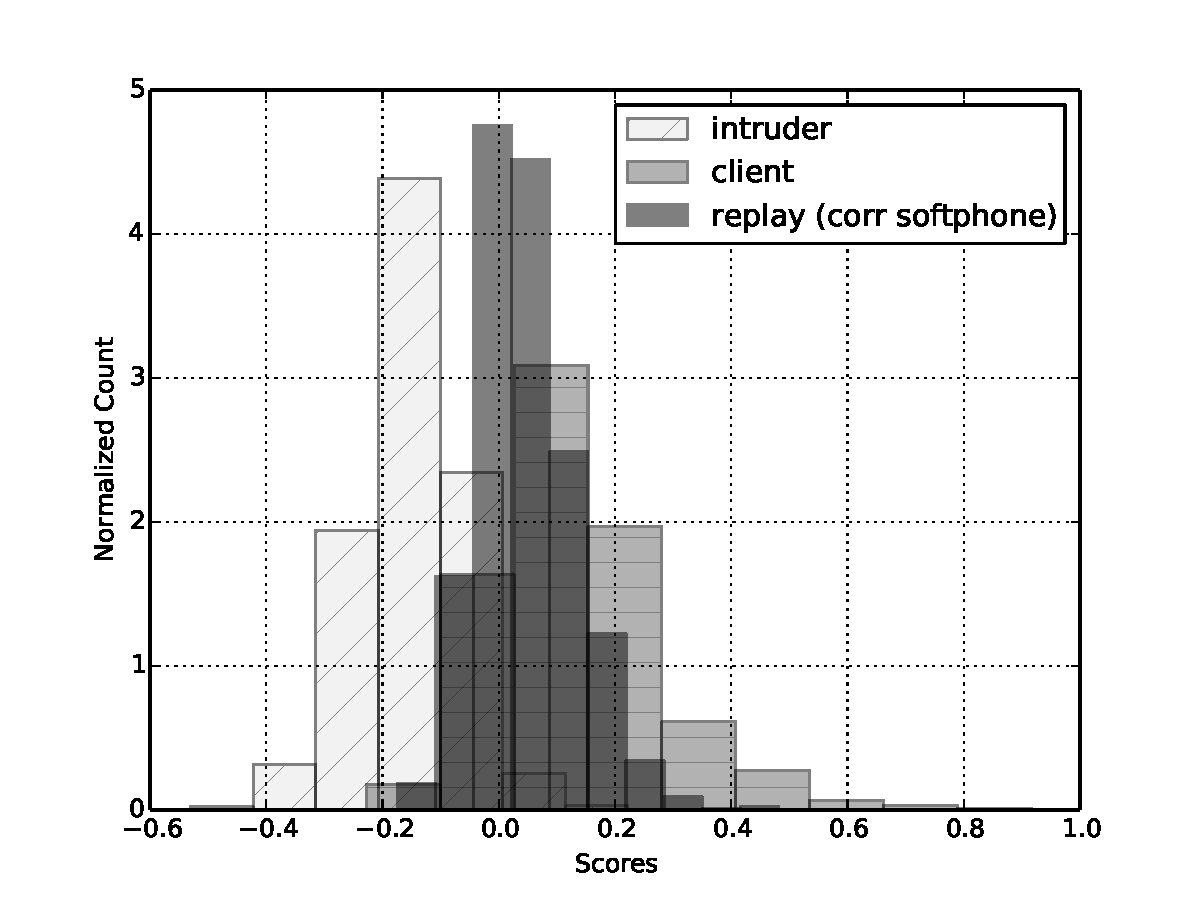
\includegraphics[width=1\linewidth]{Figs/dist_GMM_corr_iPhone.pdf}
%	\caption{DET plots for GMM-UBM (left) and i-Vectors-PLDA (right) systems.}
%	\label{fig::Dist_GMM_corr}
%	\end{minipage}


%	\begin{minipage}{0.5\textwidth}
%	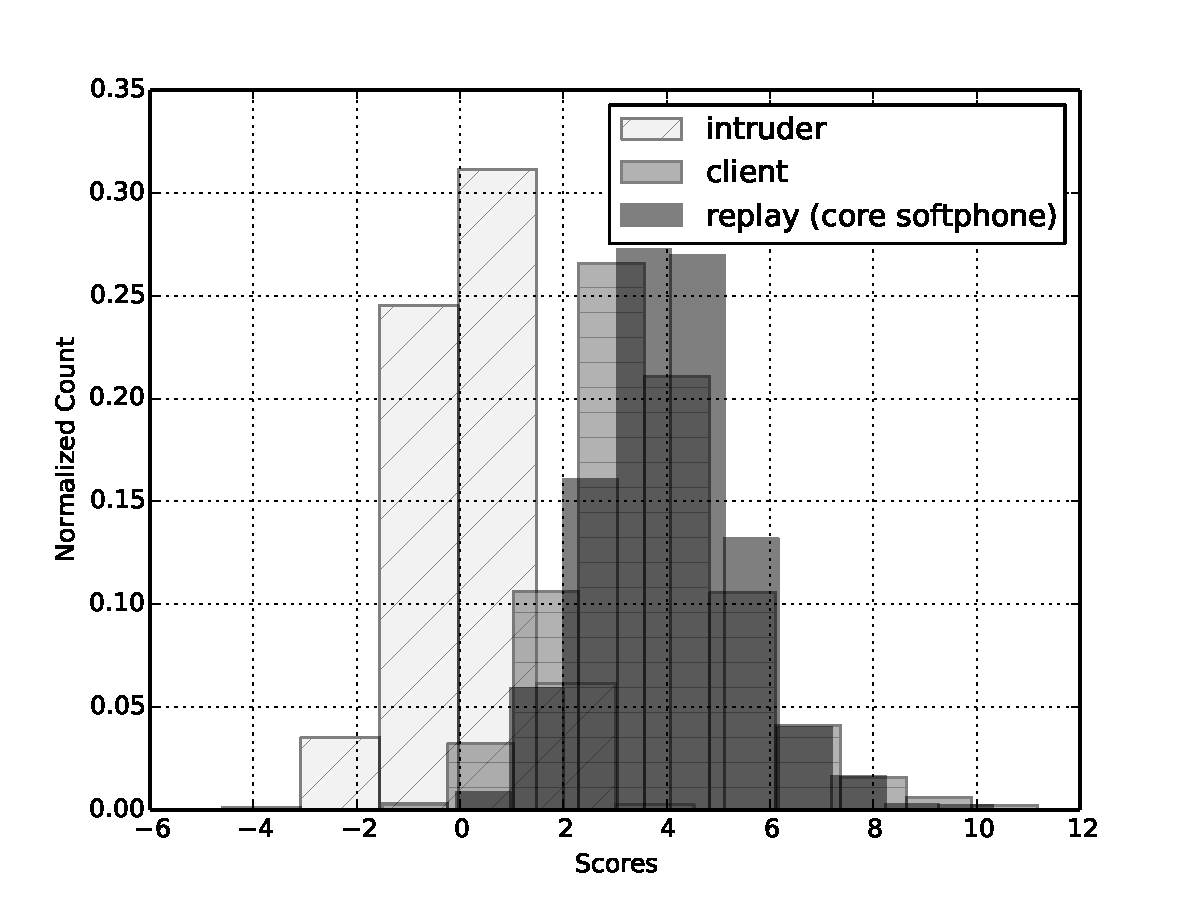
\includegraphics[width=1\linewidth]{Figs/dist_GMM_T_corr_iPhone.pdf}
%	\caption{DET plots for iVectors-PLDA xxxxxxxxxxxxxxxxxxx}
%	\end{minipage}

%	\caption{Score distribution for the GMM-UBM system without (top) and with (bottom) score normalisation.}
%	\label{fig::Dist_GMM.T_corr}

%\end{figure}



%% comparison with other attacks
\subsection{Comparison to voice conversion and speech synthesis}


%\begin{table*}[!t]
%\renewcommand{\arraystretch}{1.2}
%\begin{center}
%    \begin{tabular}{ l || c c c c c c}
%    \hline
%     	 Attack & GMM & SGL & SGL-NAP & SGL-FA & FA & IV-PLDA \\ 
% \hline \hline
%Na\"{i}ve impostor &  9.08 &  7.89 & 6.35  &  6.08 &  5.60 &  3.20 \\ 
%Replay             & 37.99 & 31.33 & 31.03 & 28.24 & 31.89 & 25.95 \\
%Voice conversion   & 31.48 & 36.94 & 30.44 & 30.23 & 23.16 & 20.45 \\ 
%Speech synthesis   & 39.90 & 14.66 & 13.83 & 11.98 & 30.81 & 10.92 \\ 
%\hline
%    \end{tabular}
%    \caption{EER values for different ASV systems for various spoofing attacks, without score normalisation.{\bfseries I missed why these results aren't in the same table as replay results - Tab.~\ref{tab::results_EER}}}
%		\label{tab::results_EER_4attacks}
%   \end{center}
%\end{table*}


\begin{figure}[!t]
	\centering
	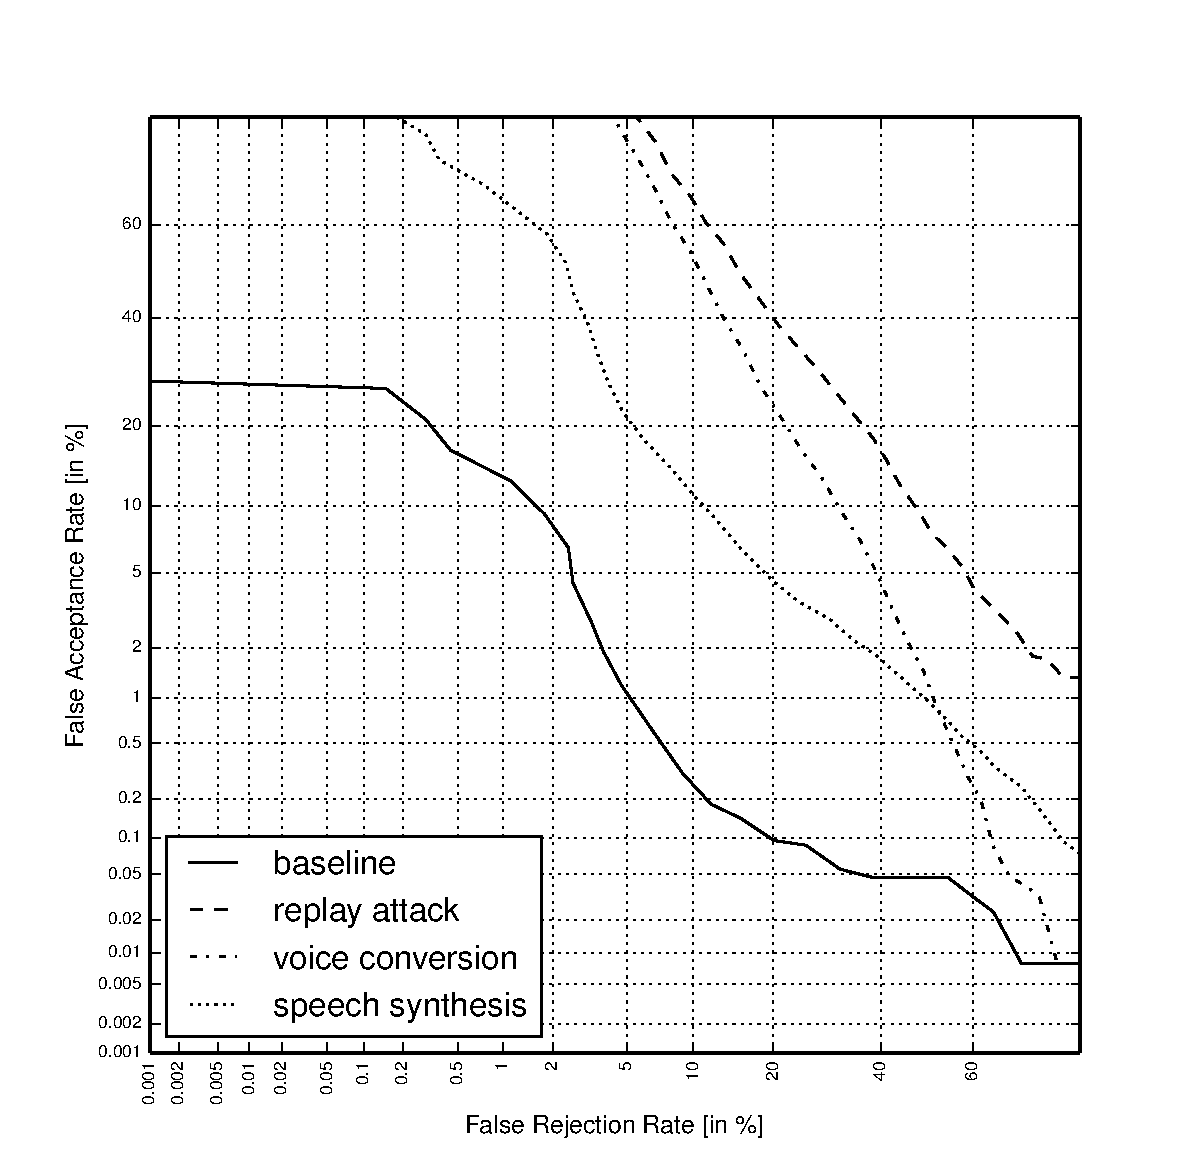
\includegraphics[width=1\linewidth]{Figs/DETs_IV_ss_vc_rp.pdf}
	\caption{DET plots for iVector-PLDA system and various attacks.}
% {\bfseries Axis keys and labels are too small.}}
	\label{fig::DETs_4attacks}
\end{figure}

DET profiles showing the vulnerabilities to replay, voice conversion and speech synthesis attacks are illustrated in Fig.~\ref{fig::DETs_4attacks} for the IV-PLDA system.  While the comparison of such profiles is not strictly meaningful\footnote{The authors are not experts in speech synthesis, nor voice conversion.  Different spoofing algorithms may well yield different comparative results. For example, other authors~\cite{DeLeon2012}, show considerably greater vulnerabilities for speech synthesis \bfseries{Do you know other papers with higher EERs for the NIST protocol? Don't we help our reviewers too much here? ;)}} it is clear that replay attacks are at least as great a threat to ASV reliability as voice conversion and speech synthesis.  This trend is consistent across the full range of ASV systems.  Again, while the comparisons are not strictly meaningful, results in rows 6 and 7 of Tab.~\ref{tab::results_EER} show the broad vulnerability of all seven ASV systems to replay attacks. {\bfseries Can add more here once figures are available.}

%To compare the reply threat with the threat of voice conversion and speech synthesis, we took the average results for all replay devices, as well as the average for office and corridor as the replay environment.
%The impact of voice conversion, despite demanding considerably more effort to implement, causes a similar degradation in performance to that of replay attacks. E.g., the SGL system yielded the EER of 37\% for voice conversion and on average 31\% for replay (see Table \ref{tab::results_EER_4attacks}); in contrast, the IV-PLDA system showed to be more resistant to voice conversion than replay (20.5\% EER vs. 26\%, respectively). 




%High-effort speech synthesis attacks proved much less effective -- the EER for the best IV-PLDA system reached less than 11\%, whilst replay attack caused an increase of the EER to 20.5\%. This confirms the results obtained during preliminary experiments (for smartphone-office combination only) described in~\cite{Alegre2014}. 




\subsection{Replay countermeasure}


\begin{table*}
\renewcommand{\arraystretch}{1.2}
\begin{center}
    \begin{tabular}{ l || c c c | c c c}
    \hline
 \multirow{2}{*}{Environment}  & \multicolumn{3}{c|}{EER (\%)} & \multicolumn{3}{c}{SFAR (\%)} \\
     	 & no CM & with FFD & with LBP & no CM & with FFD & with LBP\\ 

 \hline \hline
Office   & 30.30 & 13.62 & 9.56 & 88.70 & 63.93 & 46.29\\
Corridor & 24.53 & 11.34 & 7.00 & 80.91 & 50.25 & 30.52\\
None & 49.46 & 42.14 & 46.77 & 97.00 & 95.17 & 95.76\\
\hline
    \end{tabular}
    \caption{EER and SFAR values for various environment of replay attacks, with and without the FFD or LBP countermeasures applied, for IV-PLDA. The SFAR was measured for FRR equal to the baseline EER (2.98\%).}
		\label{tab::results_CM_rooms}
   \end{center}
\end{table*}


%\begin{table*}
%\renewcommand{\arraystretch}{1.2}
%\begin{center}
%    \begin{tabular}{ l || c c c | c c c}
%    \hline
% \multirow{2}{*}{Environment}  & \multicolumn{3}{c|}{EER (\%)} & \multicolumn{3}{c}{SFAR (\%)} \\
 %    	 & no CM & with FFD & with LBP & no CM & with FFD & with LBP\\ 
 %\hline \hline
%Smartphone   & 33.96 & 11.66 & 7.52 & 88.38 & 54.83 & 36.79\\
%Tablet & 34.48 & 11.82 & 7.50 & 88.42 & 55.33 & 36.83\\
%Stand-alone speaker & 35.84 & 13.96 & 9.83 & 89.80 & 61.11 & 41.60\\
%\hline
%    \end{tabular}
%    \caption{EER and SFAR values for various replay devices used for attacks, with and without the FFD or LBP countermeasures applied, for IV-PLDA. The SFAR was measured for FRR equal to the baseline EER (2.98\%).}
%		\label{tab::results_CM_spk}
%   \end{center}
%\end{table*}

Fig.~\ref{fig::DETs_CM} illustrates the performance of the far-field and LBP-based countermeasures for replay data collected in an office and a corridor environments. It shows directly the efficiency of spoofing detection, independently from an ASV systems. The plot illustrates that the LBP countermeasure yields much better results than the FFD one, achieving the EER of 2.87\%, while the FFD method yielded 16.53\%. The step-like shape of the DET curve for the LBP is typical to classifiers based on decision trees.

% {\bfseries Just a simple two-class classifier on its own - not integrated with the ASV systems.}

The next results show performance of the both analysed countermeasures when integrated with the IV-PLDA system. We selected this ASV, since it is the state-of-the-art, widely used ASV solution, and therefore it is likely that it can be a victim of replay spoofing. The middle two profiles in Fig.~\ref{fig::DETs_replay_IV} show the impact of the far-field detection and LBP-based countermeasures on such a system. While they show reductions in the EER compared to the upper-most profile, they remain far from the original baseline.

%Tab.~\ref{tab::results_CM_rooms} illustrates the performance of the IV-PLDA system...



%{\bfseries we need to speak about this.  It's difficult to know why you show results only for the IV-PLDA from here on.  Why not the SGL-FA system which seems to be the most robust?  I'm also wondering if we can merge tables II and III to save some space.  Probably the SFAR does not bring a great deal new to the paper beyond what the EER metrics already show. } [AJ] I have no idea how to integrate it in a clear way. Table II is for 7 ASVs, Table III concerns just the IV-PLDA... We would save space, but loose on clearness...

The detailed results of experiments with FFD and LBP countermeasures for various replay environment, averaged across the replay devices, are presented in Table~\ref{tab::results_CM_rooms}. It shows that the countermeasure performance varies depending on acoustic environment. The relative improvement caused by the countermeasures turned out to be the highest for the office -- in this case the EER decreased from 30\% down to less than 14\% for FFD and less than 10\% for LBP. Also for the corridor LBP turned out to be more effective than FFD -- 7\% EER vs. 11\%, respectively, also the SFAR result was much lower (30\% vs. 46\%). When acoustic conditions were not considered, both countermeasures performed poorly, with the EER results slightly better for FFD. 

%Table~\ref{tab::results_CM_spk} displays the results of the countermeasure experiments for various replay devices, averaged across different acoustic environments (only office and corridor were taken into account, as they are by far most realistic). Also here the LBP-based countermeasure yields better results than FFD. Both countermeasures helped most for a smartphone and a tablet (the EER values decreased to less than 12\% for FFD and to 7.5\% for LBP). The results for a stand-alone speaker are only slightly worse (14\% and 10\%, respectively), most likely due to higher quality of this device (see much better frequency response shown in Fig.~\ref{fig::IRs}). 



%% DETs w/wo CM
\begin{figure}
	\centering
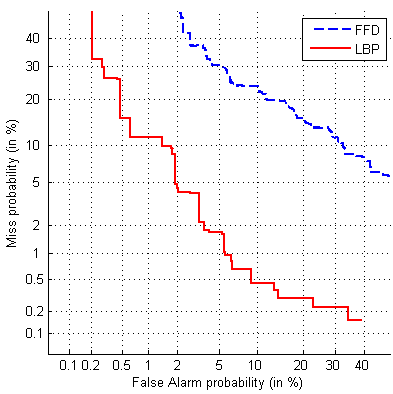
\includegraphics[width=1\linewidth]{Figs/DET_CM.png}
	\caption{DET plots for replay spoofing detection using the FFD or LBP countermeasures (measured independently from ASVs).} % {\bfseries  I suggest to replace this DET plot with an ASV-independent assessment - i.e. a pure assessment of the CM on its own.}}
	\label{fig::DETs_CM}
\end{figure}



% discussion 
\subsection{Interpretation of results}

The results presented above corroborate the findings of previous work performed with considerably smaller databases.  While reporting the first work with NIST databases and replay attacks emulated in similar fashion to all past work with voice conversion and speech synthesis, there are some aspects of the methodology which must be highlighted in order that results are sensibly interpreted.

First, the results show that replay attacks are of comparable threat to voice conversion and speech synthesis; they are not intended, nor sufficient to show that replay attacks cause the greatest degradations in ASV performance.  The relative degradations are naturally a function of the authors' effort and expertise in each approach, whereas they are not expert in voice conversion, nor speech synthesis.  Other, perhaps more sophisticated voice conversion and speech synthesis algorithms may well cause greater degradations in ASV performance than those reported here.  The work should therefore be taken as evidence only of the importance of ensuring ASV robustness to replay spoofing in the future.

These arguments lead naturally to the comparisons regarding the effort and expertise involved in the implementation of each spoofing attack.  Whereas voice conversion and speech synthesis are relatively high-effort, high-technology attacks, replay spoofing is implemented easily, without any specific expertise or equipment.  Accordingly, the threat posed by replay attacks should be considered greater in a practical perspective, even in the case that future work shows degradations in ASV performance cased by replay are lower than those caused by voice conversion and speech synthesis; they are in any case a significant threat and the most likely form of spoofing 'in the wild'.



\subsection{Future work}

There are also some aspects of the results which require further work to investigate and explain.  Of particular note is the vulnerability of the SGL system whose EER increases to 90\% when subjected to replay attacks; all other ASV systems have EERs in the order of 25\% to 50\%.  Our initial investigations have shown that score normalisation may be the cause.  Other experiments without score normalisation showed EERs of between 30\% and 50\%.  Accordingly, further work is required to study the impact of score normalisation on ASV vulnerabilities to spoofing. 

There are also some as yet unanswered questions regarding the impact of channel compensation.  The main idea behind the detection of replay attacks essentially involves the detection of unexpected channels.  Thus, while channel compensation has unquestionable utility in ensuring the usability of ASV across different devices, for example, it may also work to the fraudster's advantage; it can make the very channel characteristics needed to prevent replay attacks more difficult to detect.  There is some evidence of this in the difference between results for the IV and IV-PLDA systems.  While the latter gives better baseline performance, it is also marginally more vulnerable to replay attacks.  Further work should investigate this link.

Finally, further work should assess the threat with a more application-driven methodology.  That chosen here was motivated by the need to compare the threat of replay to that of voice conversion and speech synthesis, simply as a means of prioritising future work, i.e.\ to determine whether or not replay is a genuine threat.  While the the NIST SRE datasets were essential in order to support comparisons to other work, and are almost a requirement as regards publication, they were designed more for surveillance and security scenarios rather than authentication applications more relevant to spoofing.  Since replay spoofing is undeniably application specific, future work should thus consider more the application than the dataset.  It is stressed, however, that this criticism can be levelled equally to all of the past work.
